%!TEX TS-program = xelatex
%!TEX encoding = UTF-8 Unicode

\documentclass[border=0.0cm]{standalone}
% Pacchetti per font e colori
\usepackage{fontspec}

\usepackage{tikz}

\usepackage{Alegreya}
\usepackage{newpxmath}
%\usepackage{fourier}

\usetikzlibrary{
  decorations.text
}

\begin{document}
\begin{tikzpicture}
  \draw[color=white] (-14.4,-8.2) rectangle (14.4,8.2);
  \tikzstyle{every node}=[font=\small]
  
  \begin{scope}[rotate=3]
     \draw[very thick, ->] (-5,0) -- (5,0);
     \draw[very thick, ->] (-3,0) arc (180:2:3cm);
%    \draw[very thick, ->] (3,0) arc (0:-178:3cm);
    
    % Pallino centrale con etichetta
%    \draw[fill=black] (0,0) circle (0.1cm);
%    \node[above=3pt, font=\Large, rotate=3] at (0,0) {$m(t)$};
    
    % Pallini superiore e inferiore con etichette
%    \draw[fill=black] (0,3) circle (0.1cm);
%    \node[above=3pt, font=\Large] at (0,3) {FIR};
    
%    \draw[fill=black] (0,-3) circle (0.1cm);
%    \node[below=3pt, font=\Large] at (0,-3) {IIR};
  \end{scope}
  
  \node[anchor=south east] at (13.9,-7) {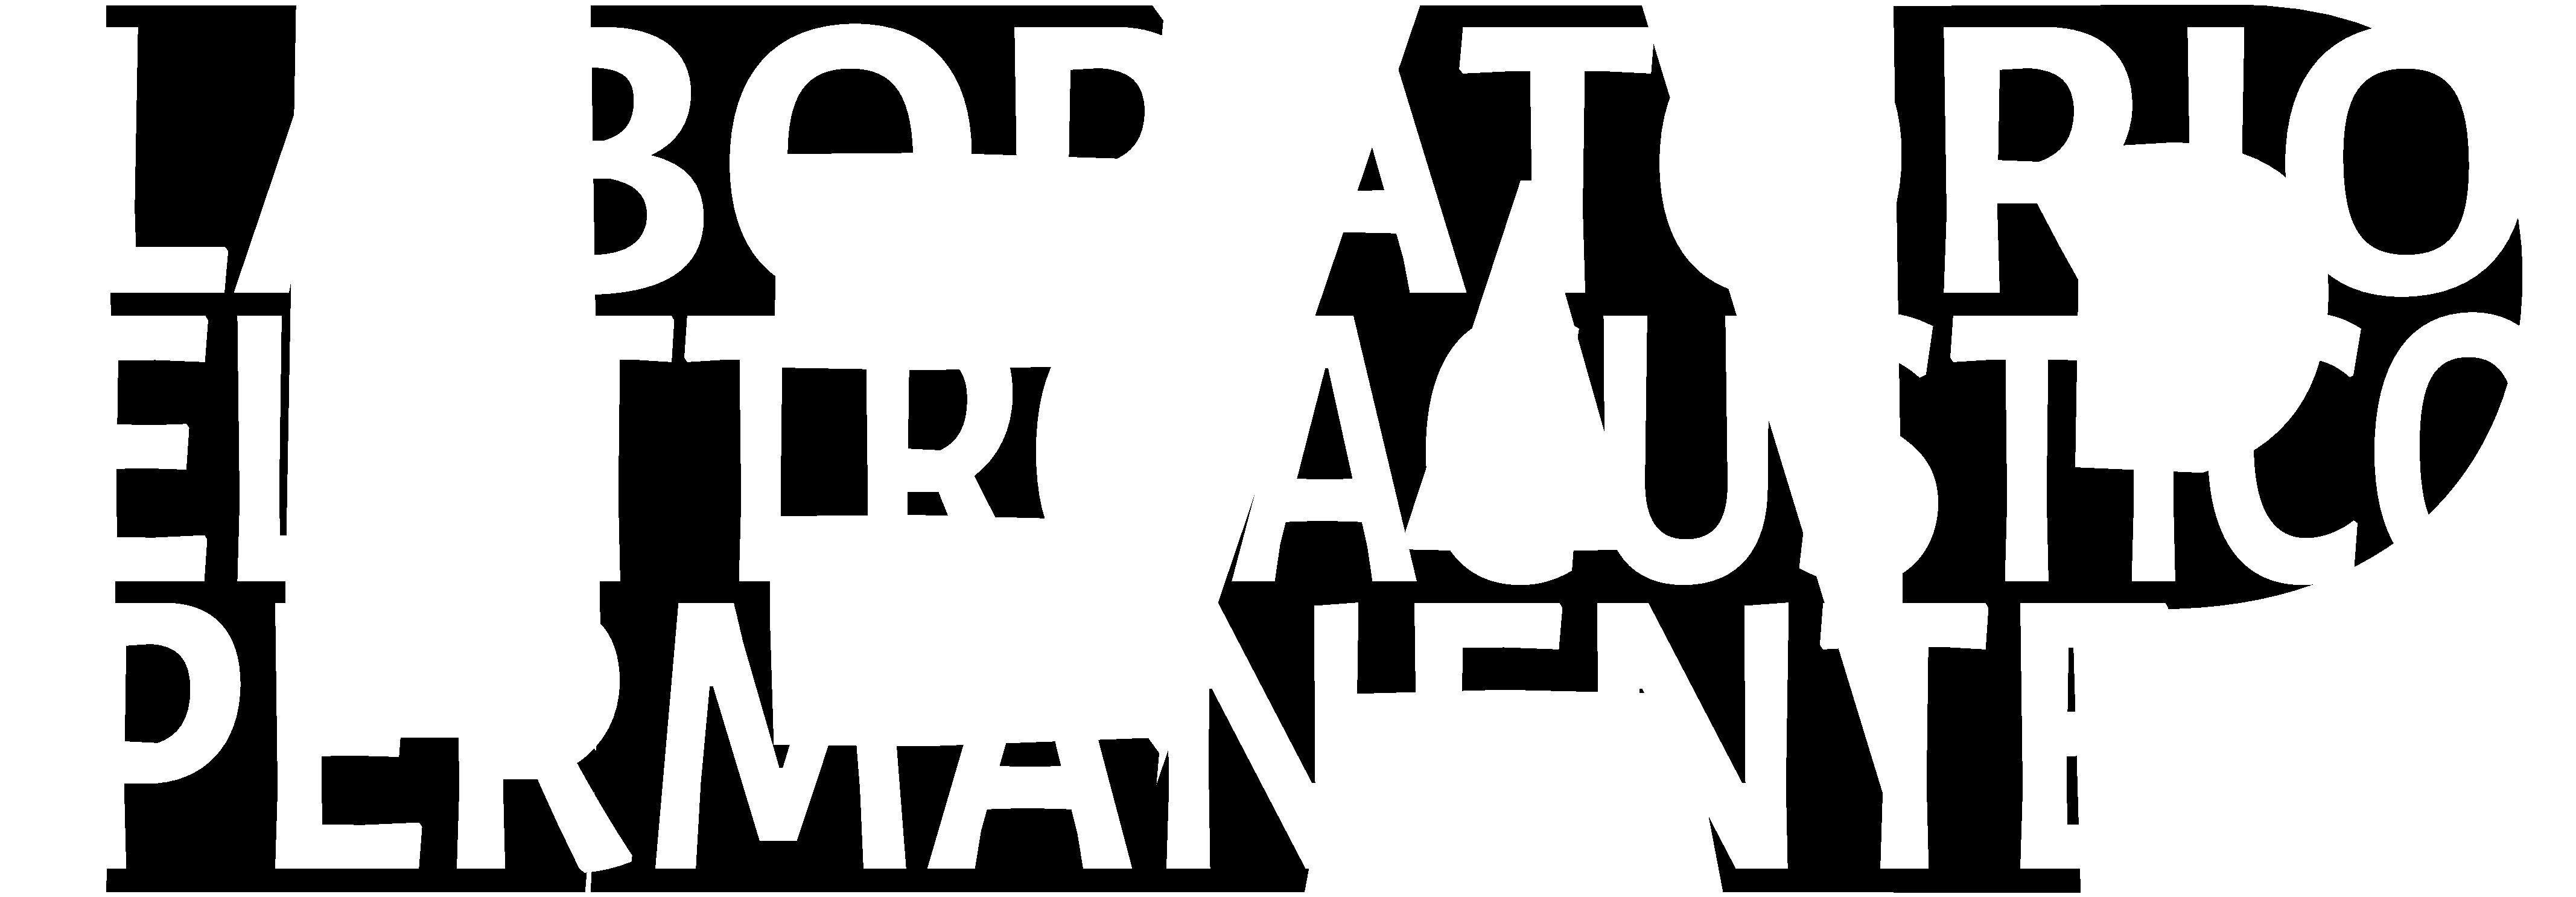
\includegraphics[width=3cm]{2023-11-12-logo-kern.pdf}};
  \node[anchor=south east] at (13.9,-8) {
\includegraphics[width=3cm]{gs-signature_a}};
\end{tikzpicture}
\end{document}

%Etimologia e radici linguistiche
%Memoria deriva dal latino memoria, sostantivo femminile che ha la sua radice nel verbo memini ("ricordare", "essere memore"). Questo verbo appartiene alla famiglia indo-europea *men-, che indica l'attività mentale del pensare e ricordare. La stessa radice si ritrova in greco antico μνήμη (mneme) e μνῆμα (mnema), da cui derivano termini come "mnemonica" e "amnesia".
%Il suffisso latino -oria indica il luogo o lo strumento dell'azione, suggerendo che memoria fosse concepita originariamente come lo "spazio mentale" dove si conservano i ricordi.

%Eredità comune: memoria come temporalizzazione creativa
%Insieme, questi autori delineano una concezione della memoria come "temporalisation créatrice" - processo attraverso cui il reale si costituisce temporalmente, conservando il passato non come dato morto ma come energia virtuale che alimenta la creazione del nuovo.
%La memoria cessa così di essere problema epistemologico (come ricordiamo?) per diventare questione ontologica (come il tempo produce realtà?).